% \documentclass{article}
% \usepackage{tikz}
% \usepackage{amsmath}

% \begin{document}
\begin{figure}
    \centering
    \resizebox{\textwidth}{!}{
    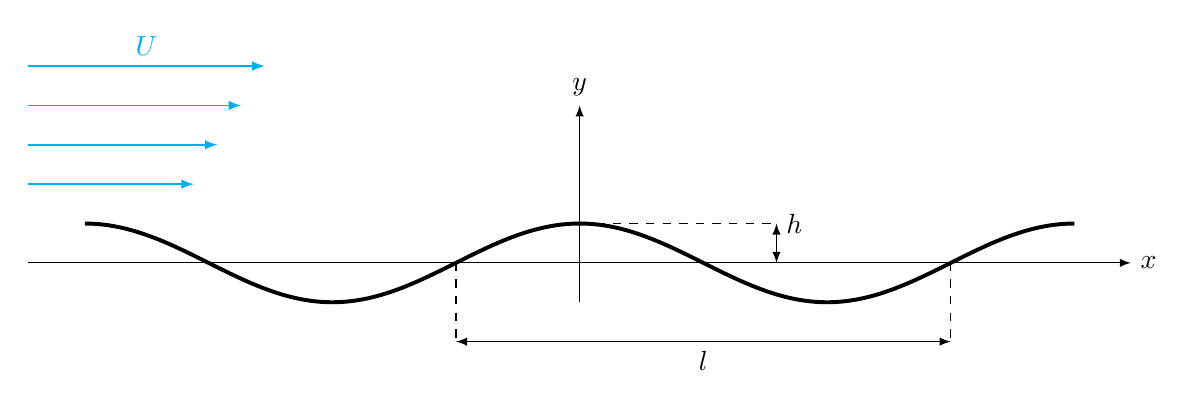
\begin{tikzpicture}[scale=1.0]
            % Achsen
        \def\startx{-7}
        \def\endx{-4}
        \def\starty{2.5}
        \def\ydis{0.5}
        \def\xenddis{0.3}
        \draw[->,>=latex] (-7, 0) -- (7, 0) node[right] {$x$};
        \draw[->,>=latex] (0, -0.5) -- (0, 2) node[above] {$y$};
        \draw[->,>=latex,cyan, line width=0.02cm] (\startx, \starty) -- (\endx, \starty) node[midway, yshift=0.25cm] {$U$};
        \draw[->,>=latex,cyan, line width=0.02cm] (\startx, \starty-\ydis) -- (\endx-\xenddis, \starty-\ydis);
        \draw[->,>=latex,cyan, line width=0.02cm] (\startx, \starty-2*\ydis) -- (\endx-2*\xenddis, \starty-2*\ydis);
        \draw[->,>=latex,cyan, line width=0.02cm] (\startx, \starty-3*\ydis) -- (\endx-3*\xenddis, \starty-3*\ydis);

        % % Gitterlinien optional
        % \draw[very thin, gray!30] (0, -1.5) grid[xstep=1, ystep=0.5] (7, 1.5);

        % Sinusfunktion
        \draw[thick, line width=0.05cm, black, domain=-2*pi:2*pi, samples=200] 
        plot (\x, {0.5*cos(\x r)});

        % Vermassungslinie l
        \def\xpos{0}
        \def\ypos{-1}
        \def\startmeas{-pi/2}
        \def\endmeas{3*pi/2}
        \draw[<->,>=latex] (\startmeas,\ypos) -- (\endmeas,\ypos) node[midway, below] {$l$};

        % Hilfslinien
        \draw[dashed] (\startmeas,\xpos) -- (\startmeas,\ypos);
        \draw[dashed] (\endmeas,\xpos) -- (\endmeas,\ypos);
        
        % Vermassungslinie h
        \def\xpos{2.5}
        \def\ypos{0}
        \def\startmeas{0}
        \def\endmeas{0.5}
        \draw[<->,>=latex] (\xpos,\startmeas) -- (\xpos,\endmeas) node[right] {$h$};

        % Hilfslinien
        \draw[dashed] (\startmeas,\endmeas) -- (\xpos,\endmeas);
        \draw[dashed] (\startmeas,\ypos) -- (\xpos,\ypos);
    \end{tikzpicture}
    }
    \caption{Strömung über einem Wellblech.}
    ~\label{fig:wellblech}
\end{figure}

% \end{document}
